\documentclass[11pt,a4paper]{article}

% ── Packages ──
\usepackage[margin=0.85in,headheight=15pt,top=0.8in,bottom=0.9in]{geometry}
\usepackage{cite}
\usepackage{amsmath,amssymb,amsfonts,amsthm}
\usepackage{bm}
\usepackage{algorithmic}
\usepackage{algorithm}
\usepackage{graphicx}
\usepackage{textcomp}
\usepackage{xcolor}
\usepackage{booktabs}
\usepackage{multirow}
\usepackage{array}
\usepackage{tabularx}
\usepackage{url}
\usepackage{hyperref}
\usepackage{listings}
\usepackage{subcaption}
\usepackage{enumitem}
\usepackage{setspace}
\usepackage{titlesec}
\usepackage{fancyhdr}
\usepackage{float}
\usepackage{tikz}
\usetikzlibrary{arrows.meta,positioning,calc}

% Clickable, colored hyperlinks for citations and URLs
\hypersetup{
  colorlinks=true,
  linkcolor=blue!60!black,
  citecolor=blue!60!black,
  urlcolor=blue!70!black,
  pdftitle={Fast PUF-Based Authentication Protocol for UAV Swarm Networks},
  pdfauthor={Md Ziyad Hussain}
}

\newtheorem{theorem}{Theorem}
\newtheorem{lemma}[theorem]{Lemma}
\newtheorem{corollary}[theorem]{Corollary}
\newtheorem{definition}{Definition}

\setstretch{1.05}

% Compact section spacing
\titlespacing*{\section}{0pt}{1.2ex plus 0.4ex minus 0.2ex}{0.6ex plus 0.2ex}
\titlespacing*{\subsection}{0pt}{0.9ex plus 0.3ex minus 0.2ex}{0.4ex plus 0.2ex}
\titlespacing*{\subsubsection}{0pt}{0.6ex plus 0.2ex minus 0.1ex}{0.3ex plus 0.1ex}
\setlist{itemsep=1pt, topsep=2pt, parsep=1pt}

\lstset{
  basicstyle=\ttfamily\small,
  breaklines=true,
  frame=single,
  numbers=left,
  numberstyle=\tiny,
  captionpos=b
}

\pagestyle{fancy}
\fancyhf{}
\rhead{\thepage}
\lhead{Fast Authentication Between UAVs}
\renewcommand{\headrulewidth}{0.4pt}

\begin{document}

% ══════════════════════════════════════════════════════════════
% TITLE PAGE
% ══════════════════════════════════════════════════════════════
\begin{titlepage}
\centering
\vspace*{0.4cm}


\includegraphics[width=2.6cm]{image.png}

\vspace{0.6cm}

{\LARGE \textbf{Indian Institute of Information Technology Guwahati}}

\vspace{0.2cm}

{\large Department of Computer Science and Engineering}

\vspace{1.6cm}

{\Huge \textbf{Fast Authentication Between UAVs}}

\vspace{0.5cm}

{\large A PUF-Based Four-Phase Swarm Authentication Protocol:\\ Design and Provable Security}

\vspace{1.8cm}

\begin{tabular}{rl}
  \textbf{Author:}     & Md Ziyad Hussain \\
  \textbf{Roll No.:}   & 2301128 \\
  \textbf{Email:}      & \texttt{ziyad.hussain23b@iiitg.ac.in} \\
  \textbf{Supervisor:} & Dr.\ Rakesh Matam \\
                       & Assistant Professor, CSE \\
\end{tabular}

\vspace{1.4cm}

{\large Indian Institute of Information Technology Guwahati}\\[0.2cm]
{\large Bongora, Assam 781015, India}\\[0.4cm]
{\large 2026}

\vfill
\end{titlepage}

% ══════════════════════════════════════════════════════════════
% ABSTRACT
% ══════════════════════════════════════════════════════════════
\setcounter{page}{1}
\begin{abstract}
\noindent
Unmanned Aerial Vehicle (UAV) swarms require authentication that is fast,
lightweight, and resilient to the physical capture of individual drones.
Traditional public-key infrastructure (RSA-2048, ECC-256) adds
millisecond-scale handshake cost on embedded processors and, more seriously,
relies on private keys stored in non-volatile memory---a liability the moment
a UAV is captured. We present a four-phase authentication protocol whose root
of trust is a Physical Unclonable Function (PUF) embedded in each UAV. The
protocol covers (1)~secure enrollment, in which a fuzzy extractor over a
BCH(255,131,18) code turns noisy PUF measurements into a \emph{stable}
per-device master key while storing no secret on the drone; (2)~UAV--Ground
Station (GS) mutual authentication in which every message is protected by a
keyed message-authentication code and the raw PUF response never leaves the
device; (3)~direct UAV--UAV peer authentication, without GS involvement,
rooted in \emph{per-pair} credentials delivered under authenticated
encryption; and (4)~session-key establishment in which a mandatory,
authenticated ephemeral Diffie--Hellman exchange provides perfect forward
secrecy. The protocol uses only a $160$-bit hash---instantiable as SHA3-256
truncated to $160$~bits or SPONGENT-160---together with a keyed MAC, a
lightweight authenticated-encryption scheme, a key-derivation function, and a
single elliptic curve, so that it fits comfortably on resource-constrained
aerial platforms. We give a complete security analysis: six theorems
covering mutual authentication in both directions, peer authentication, replay
and man-in-the-middle resistance, physical-capture resistance, session-key
secrecy, and perfect forward secrecy, each reduced to standard assumptions and
mirrored by a symbolic model in the Tamarin prover.
\end{abstract}

\textbf{Keywords:} UAV authentication, Physical Unclonable Function, PUF,
SPONGENT, SHA3, swarm security, lightweight cryptography, peer-to-peer
authentication, fuzzy extractor, BCH code, forward secrecy.

\newpage
\tableofcontents
\newpage

% ══════════════════════════════════════════════════════════════
% SECTION 1: INTRODUCTION
% ══════════════════════════════════════════════════════════════
\section{Introduction}
\label{sec:introduction}

\subsection{Background and Motivation}

Unmanned Aerial Vehicles (UAVs) have become integral to modern defense,
disaster response, precision agriculture, environmental monitoring, and public
safety. Multi-UAV \emph{swarms}---ten or more drones cooperating to surveil a
stadium, patrol a border, or search a disaster zone---are now the standard
operational unit~\cite{securing_uav_fanet}. Such swarms communicate
continuously with a Ground Station (GS) over a command-and-control link and
with one another over peer links to maintain formation, fuse sensor data, and
route around outages.

A fundamental prerequisite for any of this is \emph{mutual authentication}:
each UAV must verify the identity of its GS and of every peer before accepting
commands, sharing telemetry, or relaying messages. Without it, an adversary
can inject a rogue drone into the swarm, intercept sensitive data, issue
unauthorized flight commands, or mount man-in-the-middle attacks on inter-UAV
channels~\cite{puf_uav_cross_domain}.

\subsection{Limitations of Traditional Authentication}

Conventional options fit the UAV-swarm regime poorly. \textbf{RSA-2048 PKI}
requires several milliseconds per signature verification on embedded
processors and attaches hundreds of bytes of certificate per
handshake~\cite{puf_lightweight_uav}. \textbf{ECC-256} halves the cost but
still keeps a private key in non-volatile memory (NVM) that a captured drone
can surrender through side-channel or cold-boot
attacks~\cite{peer2peer_auth}. \textbf{Pre-shared keys} reach sub-millisecond
latency but compromise the entire swarm if any single device is captured, and
require $O(N^2)$ pairwise keys~\cite{puf_iot_strong_adversary}.
\textbf{Blockchain-based} schemes incur seconds of consensus latency,
incompatible with real-time coordination~\cite{puf_ntu}. In every case the
weakness is the same: a long-term secret \emph{stored} on a device that may
fall into an adversary's hands.

\subsection{Physical Unclonable Functions as a Solution}

A Physical Unclonable Function (PUF) is a hardware primitive that maps
challenges to responses using intrinsic, sub-nanometer manufacturing
variations unique to one integrated circuit~\cite{puf_overview}. A PUF is
\emph{unclonable} (it cannot be replicated, even by its manufacturer),
\emph{unpredictable} (responses to unseen challenges are unrelated to prior
ones), \emph{tamper-evident} (invasive probing destroys the response), and
\emph{lightweight} (an Arbiter PUF needs roughly $1{,}200$ gate equivalents).
Crucially, \emph{no key is stored}: the ``key'' is the silicon itself. This
removes the dominant attack surface of PKI and PSK schemes and is the
foundation of our design.

\subsection{Contributions of This Paper}

We present a complete four-phase PUF-based authentication framework for UAV
swarms. Its contributions are:
\begin{enumerate}[leftmargin=*]
  \item \textbf{A stable PUF-derived key with no stored secret.} Enrollment
  distils a stable per-device master key from the PUF via a fuzzy extractor;
  the drone regenerates it on demand from its PUF and \emph{public} helper
  data, so no secret ever resides in NVM.
  \item \textbf{Keyed authentication that keeps the PUF response on-device.}
  Every handshake message is authenticated with a keyed MAC under a
  PUF-derived key, and the raw PUF response is never transmitted, so it cannot
  be observed or harvested over the air.
  \item \textbf{GS-free peer authentication with per-pair trust.} Peers
  authenticate directly using \emph{per-pair} credentials delivered under
  authenticated encryption during Phase~2, so a compromised drone endangers
  only its own links.
  \item \textbf{Mandatory forward secrecy.} An authenticated ephemeral
  Diffie--Hellman exchange is folded into every session key, so a later
  compromise of long-term material cannot unlock past sessions.
  \item \textbf{A complete security analysis.} Six theorems, each reduced to
  standard cryptographic assumptions and corroborated by a mechanised Tamarin
  symbolic model, establish the protocol's authentication, secrecy, and
  capture-resistance guarantees.
\end{enumerate}

The remainder of the paper covers background (\S\ref{sec:background}), related
work (\S\ref{sec:related}), the protocol design (\S\ref{sec:protocol}), the
security analysis (\S\ref{sec:security}), a discussion of scalability and
design choices (\S\ref{sec:discussion}), and the conclusion
(\S\ref{sec:conclusion}).

% ══════════════════════════════════════════════════════════════
% SECTION 2: BACKGROUND
% ══════════════════════════════════════════════════════════════
\section{Background and Existing Technologies}
\label{sec:background}

\subsection{UAV Communication Architecture}

A UAV swarm has two communication planes. The \emph{vertical} plane connects
each UAV to the GS for commands, telemetry, and mission updates; the
\emph{horizontal} plane connects UAVs to one another for formation control and
data relay. Authentication must secure both, and it must continue to work on
the horizontal plane even when the GS link is briefly unavailable. Our design
therefore treats UAV--GS and UAV--UAV authentication as distinct phases with
distinct trust roots.

\subsection{Physical Unclonable Functions (PUFs)}

\subsubsection{PUF Fundamentals}

A PUF implements a challenge--response mapping $R = \mathrm{PUF}(C)$ that is
determined by uncontrollable fabrication variations. Two nominally identical
chips produce statistically independent responses to the same challenge
(inter-chip Hamming distance near $50\%$), while a single chip reproduces its
own response with only small deviation (intra-chip Hamming distance of a few
percent). These two properties---uniqueness and reliability---make a PUF a
per-device fingerprint that no attacker can duplicate.

\subsubsection{Types of PUFs}

Common strong PUFs include the \emph{Arbiter PUF}, which races two symmetric
delay paths and outputs a bit according to which signal arrives first, and the
\emph{Ring-Oscillator PUF}, which compares oscillator frequencies. Strong PUFs
expose an exponentially large challenge space, which is what allows a PUF to
serve as a source of many independent secrets. We assume a strong PUF with a
$128$-bit challenge space throughout.

\subsubsection{PUF Noise and Reliability}

Because a PUF measures physical quantities, its response drifts with
temperature, supply voltage, and aging, producing a bit-error rate (BER) of
typically $3$--$10\%$ between evaluations of the same challenge. A raw response
therefore cannot be used directly as a key; it must first be reconciled to a
stable value. This is the role of the fuzzy extractor
(\S\ref{subsec:bch}).

\subsection{Lightweight Cryptographic Hash Functions}

\subsubsection{SHA3-256 (Keccak)}
SHA3-256 is the NIST-standard sponge hash~\cite{sha3_standard,keccak_team}.
Truncated to $160$~bits it offers $80$-bit collision resistance and benefits
from fast, widely available software implementations, making it our
software-oriented instantiation of the abstract hash $h(\cdot)$.

\subsubsection{SPONGENT-160}
SPONGENT-160 is a lightweight sponge hash designed for hardware, occupying only
a few thousand gate equivalents~\cite{spongent_original}. It shares the
$160$-bit interface of truncated SHA3, so the protocol can switch between the
two without any structural change; SPONGENT is our hardware-oriented
instantiation.

\subsection{Fuzzy Extractors and BCH Error Correction}
\label{subsec:bch}

\subsubsection{Fuzzy Extractors}

A fuzzy extractor turns a noisy PUF response into a reproducible key using
public \emph{helper data}~\cite{bch_puf_extraction}. It is a pair of algorithms
$(\mathrm{Gen},\mathrm{Rep})$. Given an enrollment response $R$, $\mathrm{Gen}$
produces helper data $P$ and a key; given a later noisy response $R'$ and the
same $P$, $\mathrm{Rep}$ recovers the identical key whenever $R'$ is close
enough to $R$. We use the standard \emph{code-offset} construction over a
linear code $\mathsf{C}$: enrollment picks a random codeword $c$ and publishes
the offset $s = R \oplus c$; reproduction computes $c' = R' \oplus s$ and
decodes it back to $c$, so that if the Hamming distance $d_H(R,R') \le t$ the
original response $R$ is recovered exactly.

An important and often-misstated point concerns how much the public helper data
reveals. The offset $s$ does \emph{not} perfectly hide $R$; it discloses a
bounded amount of information---at most the code's redundancy, $n-k$ bits. The
correct security statement is therefore about \emph{residual min-entropy}: if
$R$ has min-entropy $m$, then $R$ retains at least $m-(n-k)$ bits of
min-entropy given $P$. A strong extractor applied to $R$ then yields a key that
is statistically close to uniform, provided the residual entropy comfortably
exceeds the key length. We make this precise in
Lemma~\ref{lem:helper} and use it to size the enrollment in
Phase~1.

\subsubsection{BCH Code Parameters}

We instantiate the code with BCH(255,131,18) over $\mathrm{GF}(2^8)$:
\begin{itemize}[leftmargin=*]
  \item \textbf{Codeword length} $n = 255$ bits;
  \item \textbf{Message length} $k = 131$ bits;
  \item \textbf{Error-correction capability} $t = 18$ bit-flips;
  \item \textbf{Minimum distance} $d = 37$;
  \item \textbf{Redundancy} $n-k = 124$ parity bits.
\end{itemize}
At a $3\%$ error rate a $128$-bit response is expected to flip
$128 \times 0.03 \approx 3.84$ bits, well within the $t=18$ correction radius,
so reproduction succeeds with overwhelming probability. Decoding uses the
standard pipeline of syndrome computation, the Berlekamp--Massey algorithm to
find the error-locator polynomial, a Chien search to locate errors, and
bit-flipping to correct them~\cite{sram_puf_bch}.

% ══════════════════════════════════════════════════════════════
% SECTION 3: RELATED WORK
% ══════════════════════════════════════════════════════════════
\section{Related Work}
\label{sec:related}

\subsection{PUF-Based Authentication for IoT and UAVs}
Early PUF authentication schemes target a single device authenticating to a
server~\cite{puf_lightweight_uav,puf_iot_strong_adversary,arbiter_puf_iot}.
They establish the PUF-plus-fuzzy-extractor pattern but do not address the
peer-to-peer coordination that a swarm needs.

\subsection{Peer-to-Peer UAV Authentication}
Peer authentication among UAVs has been studied with symmetric
credentials~\cite{peer2peer_auth} and in cross-domain
settings~\cite{puf_uav_cross_domain,puf_6g_uav}. A recurring weakness is that
peer trust is rooted in a single shared secret, so one captured node endangers
the whole mesh. Our design instead roots peer trust in \emph{per-pair}
credentials, confining the blast radius of a capture.

\subsection{Lightweight Hash Functions for Constrained Devices}
SPONGENT~\cite{spongent_original} and related lightweight
primitives~\cite{lightweight_crypto_evaluation} target minimal hardware area.
We keep a hash-agnostic interface so that a device may run SHA3 in software or
SPONGENT in hardware without changing the protocol.

\subsection{Comparison of Existing Approaches}

Table~\ref{tab:related_comparison} contrasts our design with representative
alternatives along the security features that matter for a swarm.

\begin{table}[H]
\centering
\caption{Feature Comparison of UAV/IoT Authentication Approaches}
\label{tab:related_comparison}
\small
\begin{tabular}{@{}p{3.0cm}cccccc@{}}
\toprule
\textbf{Approach} & \textbf{PUF} & \textbf{Peer} & \textbf{No stored} & \textbf{Fwd} & \textbf{Err} & \textbf{Formal} \\
                  &              & \textbf{auth} & \textbf{key}       & \textbf{sec} & \textbf{corr} & \textbf{proof} \\
\midrule
RSA-2048 PKI & No & Yes & No & Opt. & N/A & Partial \\
ECC-256 & No & Yes & No & Opt. & N/A & Partial \\
PSK (AES-GCM) & No & Yes & No & No & N/A & Partial \\
Gope~\cite{puf_lightweight_uav} & Yes & No & Yes & No & Simple & Informal \\
Li~\cite{puf_uav_cross_domain} & Yes & Partial & Yes & No & BCH & Informal \\
Khan~\cite{puf_6g_uav} & Yes & No & Yes & Yes & BCH & Informal \\
Bera~\cite{peer2peer_auth} & No & Yes & No & No & N/A & Informal \\
\textbf{This work} & \textbf{Yes} & \textbf{Yes} & \textbf{Yes} & \textbf{Yes} & \textbf{BCH} & \textbf{Games + symbolic} \\
\bottomrule
\end{tabular}
\normalsize
\end{table}

Our protocol is the only entry that simultaneously provides a PUF root of
trust, direct peer-to-peer authentication, no stored key on the device,
mandatory forward secrecy, BCH-based error correction, and a security argument
combining game-based reductions with a mechanised symbolic model.

% ══════════════════════════════════════════════════════════════
% SECTION 4: PROTOCOL DESIGN
% ══════════════════════════════════════════════════════════════
\section{Proposed Protocol Design}
\label{sec:protocol}

This section presents the four-phase protocol in full. We begin with the
threat model and design goals, fix the notation, and then specify each phase
message by message, with the mathematics of every step accompanied by a plain
explanation of what it does and why it is secure.

\subsection{Threat Model and Design Goals}

\subsubsection{Threat Model}
We consider a Dolev--Yao adversary~\cite{dolev_yao} augmented with physical
capabilities: (1)~\textbf{Network adversary}---may eavesdrop, intercept,
modify, replay, delay, or drop any wireless message; (2)~\textbf{Active
challenger}---may pose as the GS toward an honest UAV and send
adversarially chosen challenges and nonces; (3)~\textbf{Physical
capture}---may seize UAVs and read their NVM, but cannot clone PUF hardware,
since invasive probing destroys it; (4)~\textbf{Computational bounds}---a
probabilistic polynomial-time (PPT) adversary cannot invert the hash, forge a
MAC or authenticated ciphertext, break PUF unclonability, or solve the
computational Diffie--Hellman problem, except with negligible probability;
(5)~\textbf{Side channels}---standard countermeasures (constant-time
primitives, power-analysis resistance) are assumed.

\subsubsection{Design Goals}
The protocol targets: (1)~mutual authentication in both directions, verified by
keyed MACs; (2)~anonymity via rotating temporary identities;
(3)~replay and man-in-the-middle resistance through nonces, timestamps, and
transcript binding; (4)~\emph{no stored secret} on the UAV, since the master
key is regenerated from the PUF on demand; (5)~GS-free peer authentication
rooted in per-pair credentials; (6)~perfect forward secrecy through a mandatory
ephemeral key exchange; (7)~lightweight operation (only a hash, keyed MAC,
AEAD, KDF, and one elliptic curve); (8)~scalability, since the $O(N^2)$ peer
authentications are independent and parallelizable; and (9)~noise tolerance
through the BCH fuzzy extractor.

\subsection{System Model and Notation}

The system consists of one GS with ample computation and tamper-resistant
storage, and $N$ UAVs, each carrying a PUF, a lightweight processor, a radio,
and a small non-volatile memory. Table~\ref{tab:notation} lists the notation
used throughout.

\begin{table}[H]
\centering
\caption{Protocol Notation}
\label{tab:notation}
\begin{tabular}{@{}ll@{}}
\toprule
\textbf{Symbol} & \textbf{Description} \\
\midrule
$\text{UAV}_i$ & The $i$-th Unmanned Aerial Vehicle \\
$\text{GS}$ & Ground Station (enrollment and credential authority) \\
$\text{ID}_i$ & Permanent identity of $\text{UAV}_i$ (64-bit) \\
$\text{TID}_i$ & Rotating temporary identity for anonymity \\
$\text{PUF}_i$ & Physical Unclonable Function of $\text{UAV}_i$ \\
$\bm{C}_i$ & Enrollment challenge block $(C_i^{(1)},\dots,C_i^{(L)})$ \\
$R,\,R'$ & Enrollment response; noisy field response \\
$\mathsf{FE}=(\mathsf{Gen},\mathsf{Rep})$ & Fuzzy extractor (\S\ref{subsec:bch}) \\
$P_i=(s_i,\text{seed}_i)$ & \emph{Public} helper data for $\text{UAV}_i$ \\
$\text{mk}_i$ & Stable per-device master key (never stored on the UAV) \\
$\text{mk}_{\text{GS}}$ & GS-only master key for pairwise credentials \\
$\text{Cred}_{ij}$ & Per-pair credential shared by $\text{UAV}_i,\text{UAV}_j$ \\
$K^{i}_{\text{auth}}$ & UAV--GS MAC key, $=\mathsf{KDF}(\text{mk}_i;\texttt{p2\text{-}auth})$ \\
$K^{ij}_{\text{auth}}$ & Peer MAC key, $=\mathsf{KDF}(\text{Cred}_{ij};\texttt{peer\text{-}auth})$ \\
$\text{SK}_i,\,\text{SK}_{ij}$ & Session keys (Phase~2 / Phase~3) \\
$h(\cdot)$ & $160$-bit hash: SHA3-256$|_{160}$ or SPONGENT-160 \\
$\mathsf{MAC}_K(\cdot)$ & Keyed message-authentication code \\
$\mathsf{AE}.\mathsf{Enc},\mathsf{AE}.\mathsf{Dec}$ & Authenticated encryption (AEAD) \\
$\mathsf{KDF}(\cdot\,;\ell)$ & Key-derivation function with label $\ell$ \\
$g,\,g^{a},\,g^{ab}$ & Generator; ephemeral public share; DH secret \\
$N_x,\,n_x$ & Random nonces (128-bit) \\
$T_x$ & Timestamp (32-bit) \\
$\oplus,\ \|$ & Bitwise XOR; concatenation \\
\bottomrule
\end{tabular}
\end{table}

Figure~\ref{fig:overview} shows how the four phases fit together: a one-time
secure enrollment, an in-field UAV--GS handshake that also distributes peer
credentials, GS-free peer handshakes, and the session keys that result.

\begin{figure}[H]
\centering
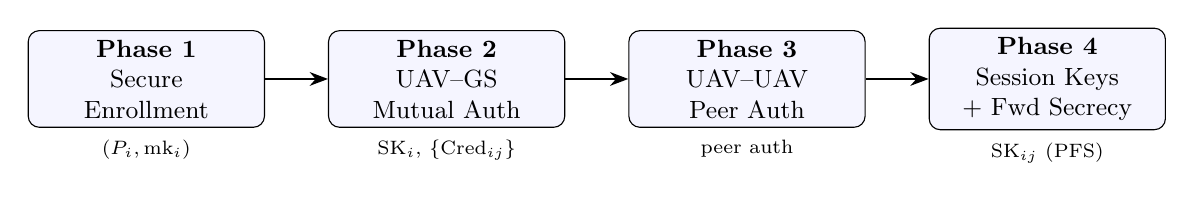
\begin{tikzpicture}[
  box/.style={draw,rounded corners,align=center,minimum height=1.15cm,
              minimum width=3.0cm,font=\small,fill=blue!4},
  >=Stealth]
\node[box] (p1) {\textbf{Phase 1}\\Secure\\Enrollment};
\node[box,right=0.8cm of p1] (p2) {\textbf{Phase 2}\\UAV--GS\\Mutual Auth};
\node[box,right=0.8cm of p2] (p3) {\textbf{Phase 3}\\UAV--UAV\\Peer Auth};
\node[box,right=0.8cm of p3] (p4) {\textbf{Phase 4}\\Session Keys\\+ Fwd Secrecy};
\draw[->,thick] (p1) -- (p2);
\draw[->,thick] (p2) -- (p3);
\draw[->,thick] (p3) -- (p4);
\node[font=\scriptsize,below=1pt of p1,align=center] {$(P_i,\text{mk}_i)$};
\node[font=\scriptsize,below=1pt of p2,align=center] {$\text{SK}_i$, $\{\text{Cred}_{ij}\}$};
\node[font=\scriptsize,below=1pt of p3,align=center] {peer auth};
\node[font=\scriptsize,below=1pt of p4,align=center] {$\text{SK}_{ij}$ (PFS)};
\end{tikzpicture}
\caption{The four phases and what each produces. Enrollment is performed once,
in a secure facility; Phases~2--4 run in the field.}
\label{fig:overview}
\end{figure}

\subsection{Phase~1: Secure Enrollment and Registration}
\label{subsec:phase1}

Enrollment runs once per UAV, in a physically secure facility over a trusted
channel (a wired link or a shielded RF cage), before the drone is deployed. Its
purpose is to establish the stable master key $\text{mk}_i$ and the public
helper data $P_i$, so that in the field the UAV can regenerate $\text{mk}_i$
from its own PUF without ever storing a secret.

\textbf{Step~1.1: PUF interrogation.}
The GS draws a block of $L$ random $128$-bit challenges
$\bm{C}_i=(C_i^{(1)},\dots,C_i^{(L)})$ and has the UAV evaluate its PUF on each:
\begin{equation}
R = \big(\,\text{PUF}_i(C_i^{(1)}),\ \dots,\ \text{PUF}_i(C_i^{(L)})\,\big).
\end{equation}
Concatenating $L$ blocks aggregates enough physical entropy to survive the
helper-data loss quantified below; $R$ is the raw enrollment response.

\textbf{Step~1.2: Key and helper-data generation.}
The GS runs the fuzzy-extractor generator $\mathsf{Gen}$ on $R$. It samples a
random seed, forms a code-offset sketch, and extracts the master key:
\begin{align}
c &= \mathsf{C}.\mathsf{Encode}(r), \quad r \xleftarrow{\$} \{0,1\}^{k}, &
s &= R \oplus c, \\[1ex]
\text{mk}_i &= \mathsf{KDF}\big(\mathsf{Ext}_{\text{seed}}(R);\ \texttt{root}\big), &
P_i &= (s,\ \text{seed}).
\end{align}
Here $s$ is the public sketch that will later let a noisy response be decoded
back to $R$, and $\mathsf{Ext}$ is a strong extractor (realised by the KDF) that
compresses $R$ into a near-uniform key. The pair $(P_i,\text{mk}_i)$ is the
output of $\mathsf{Gen}$.

\textbf{Step~1.3: Sizing the enrollment.}
Because the sketch $s$ leaks at most $n-k=124$ bits about each block
(Lemma~\ref{lem:helper}), the number of blocks $L$ is chosen so that the
entropy left after the leak still exceeds the desired key length $\ell$:
\begin{equation}
\sum_{b=1}^{L}\big(m_b-(n-k)\big)\ \ge\ \ell + 2\log(1/\varepsilon),
\label{eq:budget}
\end{equation}
where $m_b$ is the measured per-block min-entropy and $\varepsilon$ is a
negligible statistical-distance target. This inequality is what guarantees
$\text{mk}_i$ is a strong key rather than a slightly-random one.

\textbf{Step~1.4: Identity and pairwise-credential setup.}
The GS assigns a permanent identity and an initial rotating temporary identity,
and fixes a GS-only master key from which all per-pair credentials are derived:
\begin{align}
\text{TID}_i &= h(\text{ID}_i \,\|\, \text{seed}_i'), &
\text{Cred}_{ij} &= \mathsf{KDF}\big(\text{mk}_{\text{GS}};\ \texttt{pair\text{-}cred}\,\|\,\min(i,j)\,\|\,\max(i,j)\big).
\end{align}
The temporary identity hides the permanent one from eavesdroppers, and each
$\text{Cred}_{ij}$ is a distinct secret for exactly one pair. These credentials
are \emph{not} released here; they are delivered, encrypted, during Phase~2.

\textbf{Step~1.5: Storage.}
After enrollment:
\begin{itemize}[leftmargin=*]
  \item \textbf{GS stores} $\{\text{ID}_i,\ \text{TID}_i,\ \bm{C}_i,\ P_i,\ \text{mk}_i\}$ per UAV, plus the single master key $\text{mk}_{\text{GS}}$, all in tamper-resistant memory.
  \item \textbf{$\text{UAV}_i$ stores} $\{\text{TID}_i,\ \bm{C}_i,\ P_i\}$ only. Every one of these is public; \emph{no secret is stored on the drone}.
\end{itemize}
This is the central advantage of the design: capturing a UAV yields no key
material, because the master key exists only transiently, regenerated from the
PUF whenever it is needed.

\subsection{Phase~2: UAV--Ground Station Mutual Authentication}
\label{subsec:phase2}

Phase~2 runs when a UAV powers up in the field. It is a four-message exchange
that mutually authenticates the UAV and GS, establishes a forward-secret
session key $\text{SK}_i$, and delivers the UAV's per-pair credentials for
Phase~3. Both sides key their MACs with
$K^{i}_{\text{auth}}=\mathsf{KDF}(\text{mk}_i;\texttt{p2\text{-}auth})$: the GS
computes it from the stored $\text{mk}_i$, and the UAV regenerates
$\text{mk}_i$ from its PUF. Figure~\ref{fig:phase2} shows the message flow.

\begin{figure}[H]
\centering
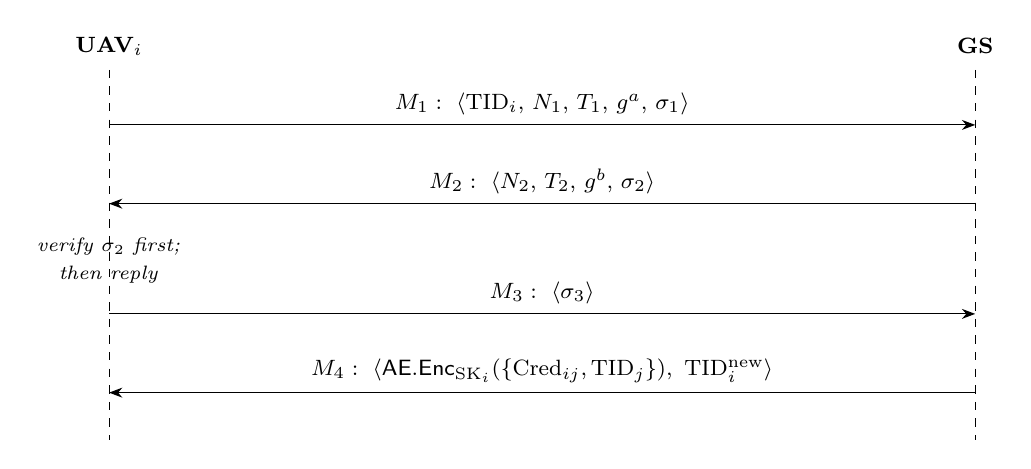
\begin{tikzpicture}[>=Stealth,font=\footnotesize]
  \node at (0,0) {\textbf{UAV$_i$}};
  \node at (11,0) {\textbf{GS}};
  \draw[dashed] (0,-0.3) -- (0,-5.0);
  \draw[dashed] (11,-0.3) -- (11,-5.0);
  \draw[->] (0,-1.0) -- node[above]{$M_1:\ \langle \text{TID}_i,\,N_1,\,T_1,\,g^{a},\,\sigma_1\rangle$} (11,-1.0);
  \draw[->] (11,-2.0) -- node[above]{$M_2:\ \langle N_2,\,T_2,\,g^{b},\,\sigma_2\rangle$} (0,-2.0);
  \node[align=left,font=\scriptsize] at (0,-2.55) {\emph{verify $\sigma_2$ first;}};
  \node[align=left,font=\scriptsize] at (0,-2.9) {\emph{then reply}};
  \draw[->] (0,-3.4) -- node[above]{$M_3:\ \langle \sigma_3\rangle$} (11,-3.4);
  \draw[->] (11,-4.4) -- node[above]{$M_4:\ \langle \mathsf{AE}.\mathsf{Enc}_{\text{SK}_i}(\{\text{Cred}_{ij},\text{TID}_j\}),\ \text{TID}_i^{\text{new}}\rangle$} (0,-4.4);
\end{tikzpicture}
\caption{Phase~2 message sequence. The UAV validates the GS's MAC before it
replies, so a fraudulent challenger receives no response; peer credentials are
delivered under authenticated encryption only after mutual authentication
succeeds.}
\label{fig:phase2}
\end{figure}

\textbf{Message~1 (Authentication request): $\text{UAV}_i \rightarrow \text{GS}$.}
The UAV picks a fresh nonce and an ephemeral Diffie--Hellman scalar, and
authenticates the opening message:
\begin{align}
N_1 &\xleftarrow{\$} \{0,1\}^{128}, \qquad a \xleftarrow{\$} \text{scalar}, \\[1ex]
\sigma_1 &= \mathsf{MAC}_{K^{i}_{\text{auth}}}\big(\texttt{M1}\,\|\,\text{TID}_i\,\|\,N_1\,\|\,T_1\,\|\,g^{a}\big), \\[1ex]
M_1 &= \langle \text{TID}_i,\ N_1,\ T_1,\ g^{a},\ \sigma_1 \rangle.
\end{align}
Because $\sigma_1$ is a MAC keyed by $K^{i}_{\text{auth}}$, only a party that
holds $\text{mk}_i$---that is, the genuine UAV (through its PUF) or the GS
(through its database)---can produce it. The tag $\texttt{M1}$ marks the
message type so that a message from one step can never be replayed as another.

\textbf{Message~2 (GS response): $\text{GS} \rightarrow \text{UAV}_i$.}
The GS checks the timestamp and the nonce for freshness, looks up
$\text{mk}_i$, verifies $\sigma_1$, and answers with its own nonce and
ephemeral share:
\begin{align}
N_2 &\xleftarrow{\$} \{0,1\}^{128}, \qquad b \xleftarrow{\$} \text{scalar}, \\[1ex]
\sigma_2 &= \mathsf{MAC}_{K^{i}_{\text{auth}}}\big(\texttt{M2}\,\|\,\text{TID}_i\,\|\,N_1\,\|\,N_2\,\|\,T_2\,\|\,g^{a}\,\|\,g^{b}\big), \\[1ex]
M_2 &= \langle N_2,\ T_2,\ g^{b},\ \sigma_2 \rangle.
\end{align}
The tag $\sigma_2$ authenticates the GS to the UAV: it binds both nonces and
both ephemeral shares under the shared key, so no network adversary can forge
or alter it.

\textbf{Message~3 (UAV confirmation): $\text{UAV}_i \rightarrow \text{GS}$.}
The UAV first regenerates its master key from its PUF and \emph{verifies
$\sigma_2$ before doing anything else}:
\begin{align}
\text{mk}_i &= \mathsf{Rep}\big(\text{PUF}_i(\bm{C}_i),\ P_i\big), \\[1ex]
&\text{abort silently if } \sigma_2 \text{ is invalid.}
\end{align}
This ``verify-before-respond'' rule is what prevents a fraudulent GS from using
the UAV as an oracle: an attacker who cannot forge $\sigma_2$ elicits no reply
at all. If the check passes, the UAV confirms the transcript:
\begin{align}
\sigma_3 &= \mathsf{MAC}_{K^{i}_{\text{auth}}}\big(\texttt{M3}\,\|\,\mathcal{T}\big), \qquad
M_3 = \langle \sigma_3 \rangle,
\end{align}
where the transcript $\mathcal{T}$ is the concatenation of all fields of $M_1$
and $M_2$. Note that the raw PUF response is consumed inside $\mathsf{Rep}$ and
\emph{never appears on the wire}; only a MAC over public values is sent.

\textbf{Message~4 (Confirmation and credential delivery): $\text{GS} \rightarrow \text{UAV}_i$.}
After verifying $\sigma_3$, both parties hold the same ingredients, so each
computes the forward-secret session key
\begin{equation}
\text{SK}_i = \mathsf{KDF}\big(\text{mk}_i \,\|\, g^{ab} \,\|\, \mathcal{T};\ \texttt{p2\text{-}sess}\big),
\label{eq:sk_p2}
\end{equation}
and the GS delivers the UAV's per-pair credentials and a fresh identity under
authenticated encryption keyed by $\text{SK}_i$:
\begin{align}
\text{CredPkg} &= \mathsf{AE}.\mathsf{Enc}_{\text{SK}_i}\big(\eta;\ \text{TID}_i;\ \{(\text{Cred}_{ij},\ \text{TID}_j)\}_{j\neq i}\big), \\[1ex]
\text{TID}_i^{\text{new}} &= h(\text{TID}_i \,\|\, \text{mk}_i \,\|\, N_1 \,\|\, N_2), \qquad
M_4 = \langle \text{CredPkg},\ \text{TID}_i^{\text{new}} \rangle.
\end{align}
Authenticated encryption gives the credentials both confidentiality and
integrity: an eavesdropper learns nothing about any $\text{Cred}_{ij}$, and a
tampered package is rejected. The session key mixes in the Diffie--Hellman
secret $g^{ab}$, which is what makes it forward-secret (Phase~4). After
Phase~2 the UAV holds $\text{SK}_i$, its peer credentials
$\{\text{Cred}_{ij}\}$, and a rotated identity.

\subsection{Phase~3: UAV-to-UAV Peer Authentication}
\label{subsec:phase3}

Phase~3 lets any two UAVs authenticate each other directly, using the per-pair
credential $\text{Cred}_{ij}$ that each received (encrypted) in Phase~2. It
needs no GS involvement, so it works even when the GS link is down. Both sides
key their MACs with
$K^{ij}_{\text{auth}}=\mathsf{KDF}(\text{Cred}_{ij};\texttt{peer\text{-}auth})$.
Figure~\ref{fig:phase3} shows the three-message flow.

\begin{figure}[H]
\centering
\begin{tikzpicture}[>=Stealth,font=\footnotesize]
  \node at (0,0) {\textbf{UAV$_i$}};
  \node at (11,0) {\textbf{UAV$_j$}};
  \draw[dashed] (0,-0.3) -- (0,-4.0);
  \draw[dashed] (11,-0.3) -- (11,-4.0);
  \draw[->] (0,-1.0) -- node[above]{$P_1:\ \langle n_i,\,T,\,g^{a'},\,\tau_1\rangle$} (11,-1.0);
  \draw[->] (11,-2.2) -- node[above]{$P_2:\ \langle n_j,\,g^{b'},\,\tau_2\rangle$} (0,-2.2);
  \draw[->] (0,-3.4) -- node[above]{$P_3:\ \langle \tau_3\rangle$} (11,-3.4);
\end{tikzpicture}
\caption{Phase~3 message sequence. Every token is a MAC keyed by the per-pair
credential $\text{Cred}_{ij}$ and tagged with its message type, so tokens
cannot be reflected or reused across steps.}
\label{fig:phase3}
\end{figure}

\textbf{Message~P1 (Peer request): $\text{UAV}_i \rightarrow \text{UAV}_j$.}
The initiator picks a fresh nonce and ephemeral share and sends an
authenticated request:
\begin{align}
n_i &\xleftarrow{\$} \{0,1\}^{128}, \qquad a' \xleftarrow{\$} \text{scalar}, \\[1ex]
\tau_1 &= \mathsf{MAC}_{K^{ij}_{\text{auth}}}\big(\texttt{P1}\,\|\,i\,\|\,j\,\|\,n_i\,\|\,T\,\|\,g^{a'}\big), \qquad
P_1 = \langle n_i,\ T,\ g^{a'},\ \tau_1 \rangle.
\end{align}
Because $\tau_1$ is keyed by $\text{Cred}_{ij}$, which only $\text{UAV}_i$ and
$\text{UAV}_j$ possess, a third party---even one holding some other pair's
credential---cannot produce it.

\textbf{Message~P2 (Peer response): $\text{UAV}_j \rightarrow \text{UAV}_i$.}
The responder verifies $\tau_1$, then answers with its own nonce and share:
\begin{align}
\tau_2 &= \mathsf{MAC}_{K^{ij}_{\text{auth}}}\big(\texttt{P2}\,\|\,i\,\|\,j\,\|\,n_i\,\|\,n_j\,\|\,g^{a'}\,\|\,g^{b'}\big), \qquad
P_2 = \langle n_j,\ g^{b'},\ \tau_2 \rangle.
\end{align}
$\tau_2$ binds both identities and both nonces, so it authenticates
$\text{UAV}_j$ to $\text{UAV}_i$ and confirms that both are in the same fresh
session.

\textbf{Message~P3 (Completion): $\text{UAV}_i \rightarrow \text{UAV}_j$.}
The initiator verifies $\tau_2$ and closes the handshake with a final tag over
the transcript $\mathcal{T}=P_1\|P_2$:
\begin{align}
\tau_3 &= \mathsf{MAC}_{K^{ij}_{\text{auth}}}\big(\texttt{P3}\,\|\,\mathcal{T}\big), \qquad
P_3 = \langle \tau_3 \rangle.
\end{align}
The three distinct type tags ($\texttt{P1},\texttt{P2},\texttt{P3}$) ensure a
token from one step can never be replayed as another, which rules out
reflection attacks. For a swarm of $N$ UAVs, full-mesh peer authentication runs
$N(N-1)/2$ independent Phase~3 exchanges (for example, $45$ for $N=10$), all of
which may proceed in parallel.

\subsection{Phase~4: Session Key Establishment and Forward Secrecy}
\label{subsec:phase4}

Phase~4 is the keying that both interactive phases finish with. In Phase~2 the
UAV--GS key is $\text{SK}_i$ of Eq.~\eqref{eq:sk_p2}; in Phase~3 the peer key is
\begin{equation}
\text{SK}_{ij} = \mathsf{KDF}\big(\text{Cred}_{ij}\,\|\,g^{a'b'}\,\|\,\mathcal{T};\ \texttt{peer\text{-}sess}\big).
\label{eq:sk_p3}
\end{equation}
Both keys have the same shape, which we write uniformly as
\begin{equation}
\text{SK} = \mathsf{KDF}\big(\underbrace{k_{\text{lt}}}_{\text{mk}_i\ \text{or}\ \text{Cred}_{ij}} \,\|\, g^{xy} \,\|\, \mathcal{T};\ \ell\big).
\label{eq:sk_unified}
\end{equation}
Two independent secrets go into every session key. The first is the long-term
key $k_{\text{lt}}$, which ties the session to the PUF (via $\text{mk}_i$) or to
the pair (via $\text{Cred}_{ij}$). The second is the ephemeral Diffie--Hellman
secret $g^{xy}$, whose public shares were authenticated inside the MAC
transcript of the corresponding handshake. Mixing in $g^{xy}$ is what provides
\emph{perfect forward secrecy}: once the ephemeral scalars are erased, an
adversary who later learns $k_{\text{lt}}$ still cannot reconstruct a past key,
because doing so would require solving Diffie--Hellman on the recorded shares.
The exchange is mandatory---there is no derivation path that omits $g^{xy}$---so
a session either establishes a forward-secret key or fails.

% ══════════════════════════════════════════════════════════════
% SECTION 5: SECURITY ANALYSIS
% ══════════════════════════════════════════════════════════════
\section{Security Analysis}
\label{sec:security}

We now analyse the protocol formally. Each theorem is proved by reducing an
attack to the violation of a standard assumption; the reductions are then
mirrored by a symbolic model (\S\ref{subsec:symbolic}).

\subsection{Assumptions}
\label{subsec:assumptions}

The proofs rely on the following standard assumptions.
\begin{enumerate}[leftmargin=*]
  \item \textbf{Hash security.} $h$ is pre-image, second-pre-image, and
  collision resistant; in the reductions it is modelled as a random oracle.
  \item \textbf{MAC unforgeability.} $\mathsf{MAC}$ is existentially unforgeable
  under chosen-message attack (EUF-CMA): without the key, a fresh valid tag can
  be produced only with negligible probability.
  \item \textbf{AEAD security.} $\mathsf{AE}$ provides ciphertext
  indistinguishability (IND-CCA) and ciphertext integrity (INT-CTXT).
  \item \textbf{PUF unpredictability.} Given polynomially many
  challenge--response pairs, the response to a fresh challenge is
  computationally indistinguishable from uniform to an adversary that does not
  possess the device; invasive probing destroys the PUF.
  \item \textbf{Diffie--Hellman.} The gap computational Diffie--Hellman
  (gap-CDH) problem is hard in $\mathbb{G}$.
\end{enumerate}

We first record the helper-data property that underpins the strength of the
master key.

\begin{lemma}[Helper-data privacy]
\label{lem:helper}
Let the enrollment response $R$ have conditional min-entropy $\widetilde{H}_\infty(R)=m$.
The code-offset sketch $s=R\oplus c$ discloses at most $n-k$ bits, so
\begin{equation}
\widetilde{H}_\infty\big(R \mid P\big)\ \ge\ m-(n-k).
\end{equation}
Consequently, if the extractor output length $\ell$ satisfies
$\ell \le m-(n-k)-2\log(1/\varepsilon)$, then $\text{mk}$ is within statistical
distance $\varepsilon$ of uniform given the public helper data $P$.
\end{lemma}

\begin{proof}
Given the internal randomness $r$, the sketch $s=R\oplus c$ is a deterministic
function of $R$ that pins $R$ to a coset of the $[n,k]$ code $\mathsf{C}$;
revealing that coset fixes at most $n-k$ syndrome bits, so by the chain rule for
average min-entropy $\widetilde{H}_\infty(R\mid s)\ge \widetilde{H}_\infty(R)-(n-k)$, and the seed is
independent of $R$. Applying the strong-extractor property to the residual
source gives a key within distance $\varepsilon$ of uniform. \hfill$\square$
\end{proof}

\subsection{Phase~2: Mutual Authentication}

\begin{theorem}[Phase~2 mutual authentication]
\label{thm:mutual_auth}
After a successful Phase~2 exchange, $\text{UAV}_i$ and the GS have mutually
authenticated one another, and both agree on the transcript $\mathcal{T}$,
except with negligible probability.
\end{theorem}

\begin{proof}
Both directions rest on the MAC key $K^{i}_{\text{auth}}=\mathsf{KDF}(\text{mk}_i;\texttt{p2\text{-}auth})$,
which by Lemma~\ref{lem:helper} and PUF unpredictability is unknown to any
adversary lacking either the PUF or the GS database.
\emph{(GS authenticates UAV.)} The GS accepts only if $\sigma_1$ (and later
$\sigma_3$) verifies under $K^{i}_{\text{auth}}$; producing a fresh valid tag
without the key is exactly an EUF-CMA forgery.
\emph{(UAV authenticates GS.)} Symmetrically, the UAV accepts only if $\sigma_2$
verifies; although every field inside $\sigma_2$ is public, the \emph{key} is
secret, so a fresh valid $\sigma_2$ is again a forgery.
A nonce collision that could enable transcript reuse occurs with probability at
most $q^2/2^{128}$ for $q$ sessions. Absent forgery and collision, the two
accepting parties share identical fields in $M_1$ and $M_2$, i.e.\ they agree on
$\mathcal{T}$. \hfill$\square$
\end{proof}

\begin{corollary}[No PUF read-out oracle]
\label{cor:oracle}
An adversary that impersonates the GS learns no PUF response, so it cannot
harvest challenge--response pairs to model the PUF.
\end{corollary}

\begin{proof}
By the verify-before-respond rule, the UAV emits $M_3$ only after $\sigma_2$
verifies, which by Theorem~\ref{thm:mutual_auth} an adversary can force only by
forging a MAC. When the check fails the UAV sends nothing; when it passes, the
only value on the wire is $\sigma_3$, a MAC over public transcript fields---the
PUF response is consumed inside $\mathsf{Rep}$ and is never transmitted. Hence
no challenge--response pair is exposed. \hfill$\square$
\end{proof}

\subsection{Replay Attack Resistance}

\begin{theorem}[Replay resistance]
\label{thm:replay}
Phase~2 and Phase~3 resist replay attacks.
\end{theorem}

\begin{proof}
Three mechanisms combine. First, every message carries a fresh $128$-bit nonce
and a timestamp verified within a window $\Delta T$; a verbatim replay reuses a
stale nonce or timestamp and is rejected. Second, each MAC binds a per-message
type tag ($\texttt{M1},\dots,\texttt{P3}$), so a token from one step cannot be
accepted at another. Third, from the second message onward each MAC binds the
partner's nonce, so a token from one session cannot be reused in another without
producing a mismatch---which, by Theorems~\ref{thm:mutual_auth}
and~\ref{thm:peer_auth}, would require a forgery. \hfill$\square$
\end{proof}

\subsection{Phase~3: Peer Mutual Authentication}

\begin{theorem}[Peer mutual authentication]
\label{thm:peer_auth}
After a successful Phase~3 exchange, $\text{UAV}_i$ and $\text{UAV}_j$ have
mutually authenticated one another, without GS involvement, and no per-pair
secret is exposed in transit.
\end{theorem}

\begin{proof}
The credential $\text{Cred}_{ij}$ reaches each endpoint only inside the Phase~2
package $\mathsf{AE}.\mathsf{Enc}_{\text{SK}_i}(\cdots)$; by INT-CTXT the
adversary cannot make a UAV accept a substituted credential, and by IND-CCA it
learns nothing about $\text{Cred}_{ij}$. Given a secret $\text{Cred}_{ij}$, the
tokens $\tau_1,\tau_2,\tau_3$ are MACs under
$K^{ij}_{\text{auth}}$; each binds both identities and both nonces, so a fresh
acceptance forces a matching computation by the partner---otherwise an EUF-CMA
forgery. Because credentials are pair-specific, a third party holding some other
$\text{Cred}_{k\ell}$ has no information about $\text{Cred}_{ij}$ and cannot
assert identity $i$ to $j$. \hfill$\square$
\end{proof}

\subsection{Man-in-the-Middle Resistance}

\begin{theorem}[MITM resistance]
\label{thm:mitm}
The protocol resists active man-in-the-middle attacks in both Phase~2 and
Phase~3.
\end{theorem}

\begin{proof}
Every accepted message is a MAC (or an authenticated ciphertext) over a
transcript that includes fresh nonces, a timestamp, a type tag, and---from the
second message onward---the partner's nonce and ephemeral share. Altering any
field invalidates the covering tag, and forging a new tag requires the secret
key (EUF-CMA / INT-CTXT). By the agreement guarantees of
Theorems~\ref{thm:mutual_auth} and~\ref{thm:peer_auth}, both endpoints therefore
hold the identical transcript, so an interposed adversary cannot sit undetected
between them. \hfill$\square$
\end{proof}

\subsection{Session-Key Secrecy and Forward Secrecy}

\begin{theorem}[Session-key secrecy]
\label{thm:key_secrecy}
For an adversary that corrupts neither endpoint of the target session, the
session key of Eq.~\eqref{eq:sk_unified} is indistinguishable from uniform.
\end{theorem}

\begin{proof}
The key is $\mathsf{KDF}(k_{\text{lt}}\|g^{xy}\|\mathcal{T})$. Two independent
secrets protect it: the long-term key $k_{\text{lt}}$
($\text{mk}_i$ by Lemma~\ref{lem:helper} and PUF unpredictability, or
$\text{Cred}_{ij}$ by IND-CCA of its delivery, Theorem~\ref{thm:peer_auth}) and
the Diffie--Hellman secret $g^{xy}$. Modelling the KDF as a pseudorandom
function, replacing it by a random function is undetectable up to its PRF
advantage; the input $g^{xy}$ is unpredictable under gap-CDH given only the
authenticated shares $g^{x},g^{y}$. Hence the output is uniform up to negligible
terms. \hfill$\square$
\end{proof}

\begin{theorem}[Perfect forward secrecy]
\label{thm:pfs}
If the ephemeral scalars are erased after use, then revealing the long-term
secrets ($\text{mk}_i$, $\text{Cred}_{ij}$, or $\text{mk}_{\text{GS}}$)
\emph{after} a target session closes does not compromise that session's key.
\end{theorem}

\begin{proof}
A post-session reveal gives the adversary $k_{\text{lt}}$ but not the erased
scalars $x,y$. The key of Eq.~\eqref{eq:sk_unified} still depends on $g^{xy}$,
which the adversary must now compute from the recorded, authenticated shares
$g^{x},g^{y}$---a gap-CDH instance. Because the ephemeral exchange is mandatory,
there is no non-ephemeral key to fall back on. Hence past keys remain
indistinguishable from uniform. \hfill$\square$
\end{proof}

\subsection{Physical Capture Resistance}

\begin{theorem}[Physical capture resistance]
\label{thm:capture}
Capturing $\text{UAV}_k$ and reading its NVM does not let the adversary
impersonate any other UAV to the GS, nor impersonate any peer pair that does not
involve $k$. A captured node's peer exposure is limited to its own $N-1$ links.
\end{theorem}

\begin{proof}
The NVM of $\text{UAV}_k$ holds only $\{\text{TID}_k,\ \bm{C}_k,\ P_k,\ \{\text{Cred}_{kj}\}_j\}$
plus any live session keys; all of $\text{TID}_k,\bm{C}_k,P_k$ are public.
Impersonating $\text{UAV}_m$ ($m\neq k$) in a fresh Phase~2 needs
$K^{m}_{\text{auth}}=\mathsf{KDF}(\text{mk}_m;\cdot)$; but $\text{mk}_m$ is never
stored, is not recoverable from $k$'s silicon (tamper evidence), and is
unpredictable (PUF assumption), so this reduces to a MAC forgery. Impersonating
a pair $(m,\ell)$ with $k\notin\{m,\ell\}$ needs
$\text{Cred}_{m\ell}=\mathsf{KDF}(\text{mk}_{\text{GS}};\cdot)$, which is
independent of every captured $\text{Cred}_{kj}$ (distinct KDF inputs, and
$\text{mk}_{\text{GS}}$ never leaves the GS). Only pairs that include $k$ share a
captured credential, giving the stated $N-1$ exposure. \hfill$\square$
\end{proof}

\subsection{Symbolic Verification}
\label{subsec:symbolic}

The computational theorems are corroborated by a symbolic model in the Tamarin
prover~\cite{tamarin}, whose multiset-rewriting calculus expresses freshness,
stateful credential issuance, and device-compromise events natively. In the
model, $h,\mathsf{MAC},\mathsf{AE},\mathsf{KDF}$ are function symbols with the
usual equational theory, each PUF is a private per-device function, and helper
data and all wire terms are public. The Dolev--Yao adversary controls the
network; two extra rules model compromise---one that reveals a captured node's
NVM (its identities, helper data, and per-pair credentials, but neither its PUF
nor its master key) and one that reveals long-term secrets after a session
closes, for the forward-secrecy query. The prover discharges lemmas that
correspond one-to-one with the theorems above: injective agreement for Phase~2
and Phase~3 (Theorems~\ref{thm:mutual_auth} and~\ref{thm:peer_auth}), a
no-replay lemma (Theorem~\ref{thm:replay}), a capture-isolation lemma
(Theorem~\ref{thm:capture}), a session-key-secrecy lemma
(Theorem~\ref{thm:key_secrecy}), and a forward-secrecy lemma
(Theorem~\ref{thm:pfs}). The PUF's noise is idealised as a noiseless private
function---its error tolerance is the computational correctness property of the
fuzzy extractor---and confidential delivery is abstracted by a symmetric
encryption operator, leaving the fine-grained secrecy argument to the
computational analysis.

\subsection{Summary of Security Properties}

Table~\ref{tab:security_summary} summarises the guarantees and the mechanism
behind each.

\begin{table}[H]
\centering
\caption{Summary of Security Properties}
\label{tab:security_summary}
\begin{tabular}{@{}p{4.6cm}cp{6.0cm}@{}}
\toprule
\textbf{Property} & \textbf{Result} & \textbf{Mechanism} \\
\midrule
UAV--GS mutual auth & Thm~\ref{thm:mutual_auth} & Keyed MAC under PUF-derived $\text{mk}_i$ \\
No PUF read-out oracle & Cor~\ref{cor:oracle} & Verify-before-respond; response stays on-device \\
Replay resistance & Thm~\ref{thm:replay} & Nonces + timestamps + type tags \\
Peer mutual auth & Thm~\ref{thm:peer_auth} & Per-pair credential + keyed MAC \\
MITM resistance & Thm~\ref{thm:mitm} & Transcript-binding MACs / AEAD \\
Session-key secrecy & Thm~\ref{thm:key_secrecy} & KDF over long-term key and DH secret \\
Perfect forward secrecy & Thm~\ref{thm:pfs} & Mandatory authenticated ephemeral DH \\
Physical-capture resistance & Thm~\ref{thm:capture} & No stored key; per-pair credentials \\
Identity anonymity & --- & Rotating temporary identities \\
\bottomrule
\end{tabular}
\end{table}

% ══════════════════════════════════════════════════════════════
% SECTION 6: DISCUSSION
% ══════════════════════════════════════════════════════════════
\section{Discussion}
\label{sec:discussion}

\subsection{Scalability}
Phase~2 is $O(N)$ in the swarm size and fully parallel across UAVs, since each
UAV's handshake with the GS is independent. Phase~3 is $O(N^2)$: full-mesh peer
authentication runs $N(N-1)/2$ exchanges (for example $45$ for $N=10$ and $190$
for $N=20$), but these too are mutually independent and can proceed in
parallel, and a deployment that only needs neighbours may authenticate a subset
of pairs. Because every operation is symmetric---a hash, a MAC, an AEAD, a KDF,
and one ephemeral exchange---per-message cost is small and does not grow with
the swarm.

\subsection{Design Choices}
Three choices give the protocol its character. First, deriving a \emph{stable}
key from the PUF means the drone stores no secret and can re-authenticate any
number of times from a single enrollment, rather than consuming a limited pool
of challenge--response pairs. Second, rooting Phase~3 in \emph{per-pair}
credentials---rather than one swarm-wide secret---means a captured node
endangers only its own links, matching the capture threat that motivates PUFs
in the first place. Third, making the ephemeral exchange \emph{mandatory} rather
than optional means forward secrecy is a property of every session, not a
feature that can be silently skipped.

\subsection{Noise Tolerance}
The BCH(255,131,18) fuzzy extractor corrects up to $18$ bit-flips, comfortably
above the $\approx 3.84$ expected flips in a $128$-bit response at a $3\%$ error
rate, so reproduction of $\text{mk}_i$ succeeds with overwhelming probability
across the temperature and voltage range of normal operation. The enrollment is
sized by Eq.~\eqref{eq:budget} so that the extracted key retains full strength
after the public helper data is accounted for.

\subsection{Limitations and Future Work}
The analysis here is at the protocol level; a mechanised end-to-end proof and a
hardware prototype are natural next steps, as is an empirical study of the PUF's
reliability across environmental extremes. Extending the model to dynamic swarm
membership (join and leave during flight) and to mobility-induced link changes
is left for future work.

% ══════════════════════════════════════════════════════════════
% SECTION 7: CONCLUSION
% ══════════════════════════════════════════════════════════════
\section{Conclusion}
\label{sec:conclusion}

We presented a four-phase PUF-based authentication protocol for UAV swarms. Its
root of trust is a stable key distilled from each drone's PUF by a fuzzy
extractor, so that no secret is ever stored on the device. Every handshake
message is protected by a keyed MAC, and the raw PUF response never leaves the
UAV, which closes the challenge-harvesting avenue that undermines naive PUF
protocols. Peer authentication runs directly between UAVs, rooted in per-pair
credentials delivered under authenticated encryption during the UAV--GS
handshake, so a captured node compromises only its own links. Every session key
folds in a mandatory, authenticated ephemeral Diffie--Hellman secret, giving
perfect forward secrecy. We proved six security theorems---mutual authentication
in both directions, peer authentication, replay and man-in-the-middle
resistance, physical-capture resistance, session-key secrecy, and perfect
forward secrecy---by reduction to standard assumptions, and mirrored them in a
Tamarin symbolic model. Built from a $160$-bit hash, a keyed MAC, a lightweight
AEAD, a KDF, and a single elliptic curve, the protocol is well matched to the
resource constraints of aerial platforms. A reference implementation and
simulation study are the subject of ongoing work.

\section*{Acknowledgment}
The author thanks the Indian Institute of Information Technology Guwahati for
providing the research infrastructure and Dr.\ Rakesh Matam for his guidance.

% ══════════════════════════════════════════════════════════════
% REFERENCES
% ══════════════════════════════════════════════════════════════
\begin{thebibliography}{25}

\bibitem{securing_uav_fanet}
A.~Mukherjee, S.~Bose, A.~Mukherjee, and S.~Saha, ``Securing UAV Flying Ad Hoc Wireless Networks: Authentication Development for Robust Communications,'' \textit{IEEE Access}, vol.~12, pp.~1--15, 2024.

\bibitem{puf_lightweight_uav}
P.~Gope and B.~Sikdar, ``A PUF-based lightweight authentication and key agreement protocol for smart UAV networks,'' \textit{IET Communications}, vol.~16, no.~18, pp.~2136--2148, 2022.

\bibitem{peer2peer_auth}
T.~Bera, S.~Das, and A.~K.~Das, ``Secure and Efficient Peer2Peer Authentication-Attestation Protocol for UAV Networks,'' in \textit{Proc. IEEE INFOCOM Workshop}, 2023, pp.~1--6.

\bibitem{puf_ntu}
National Technological University, ``PUF-Based Lightweight Security Framework for Drone Networks,'' DR-NTU Technical Report Series, 2023.

\bibitem{bch_puf_extraction}
J.~Delvaux, D.~Gu, I.~Verbauwhede, M.~Hiller, and M.-D.~Yu, ``Cryptographic Key Generation from PUF Data Using Efficient Fuzzy Extractors,'' \textit{IEEE Trans. Inf. Forensics Security}, vol.~15, pp.~2025--2038, 2020.

\bibitem{sram_puf_bch}
L.~Zhang, Y.~Li, Z.~Wang, and C.~Chen, ``SRAM-PUF Key Extraction Method and Performance Analysis Based on RS and BCH Codes,'' \textit{Electronics}, vol.~12, no.~4, p.~1012, 2023.

\bibitem{helper_data_masking}
R.~Maes, ``Helper Data Masking for Physically Unclonable Function-Based Key Generation,'' \textit{Cryptology ePrint Archive}, Report 2019/688, 2019.

\bibitem{puf_iot_strong_adversary}
U.~Chatterjee, R.~S.~Chakraborty, and D.~Mukhopadhyay, ``PUF-based Authentication in IoT against Strong Physical Adversary,'' in \textit{Proc. IEEE DATE}, 2022, pp.~1--6.

\bibitem{puf_uav_cross_domain}
B.~Li, H.~Zhu, J.~Shen, and T.~Li, ``PUF-Based Secure and Efficient Anonymous Authentication Protocol for UAV Towards Cross-Domain Environments,'' \textit{IEEE Trans. Veh. Technol.}, vol.~72, no.~9, pp.~12101--12115, 2023.

\bibitem{puf_overview}
A.~Alkatheiri, Y.~G.~Alghamdi, and S.~U.~Jan, ``Review of Physically Unclonable Functions (PUFs): Structures, Models, and Algorithms,'' \textit{Frontiers in Electronics}, vol.~4, p.~1123456, 2023.

\bibitem{puf_key_exchange}
R.~Aman, K.~Z.~Ghafoor, and S.~K.~Sood, ``PUF based Lightweight Authentication and Key Exchange Protocol for IoT,'' in \textit{Proc. IEEE GLOBECOM}, 2022, pp.~1--6.

\bibitem{puf_6g_uav}
S.~Khan, A.~Irshad, S.~A.~Chaudhry, and M.~Alazab, ``A Provably Secure and Lightweight PUF-Based Authentication Scheme for 6G-Enabled UAV Networks,'' \textit{IEEE Internet of Things J.}, vol.~11, no.~5, pp.~8532--8543, 2024.

\bibitem{arbiter_puf_iot}
L.~Xu, X.~Wang, Q.~Li, and H.~Wang, ``An Enhanced Event-Based Dynamic Authentication Protocol Leveraging Arbiter PUF for IoT Devices,'' \textit{IEEE Internet of Things J.}, vol.~10, no.~18, pp.~16123--16135, 2023.

\bibitem{lightweight_crypto_evaluation}
T.~Eisenbarth \textit{et al.}, ``Design and Evaluation of Lightweight Cryptographic Primitives for Constrained Devices,'' \textit{J. Cryptographic Engineering}, vol.~12, no.~3, pp.~245--260, 2022.

\bibitem{spongent_original}
A.~Bogdanov, M.~Kne\v{z}evi\'c, G.~Leander, D.~Toz, K.~Varici, and I.~Verbauwhede, ``SPONGENT: A Lightweight Hash Function,'' in \textit{Proc. CHES 2011}, Springer LNCS, vol.~6917, pp.~312--325, 2011.

\bibitem{sha3_standard}
National Institute of Standards and Technology (NIST), ``SHA-3 Standard: Permutation-Based Hash and Extendable-Output Functions,'' FIPS~202, 2015.

\bibitem{keccak_team}
G.~Bertoni, J.~Daemen, M.~Peeters, and G.~Van~Assche, ``The Keccak Reference,'' Version 3.0, 2011.

\bibitem{dolev_yao}
D.~Dolev and A.~Yao, ``On the Security of Public Key Protocols,'' \textit{IEEE Trans. Inf. Theory}, vol.~29, no.~2, pp.~198--208, 1983.

\bibitem{dodis_fuzzy}
Y.~Dodis, R.~Ostrovsky, L.~Reyzin, and A.~Smith, ``Fuzzy Extractors: How to Generate Strong Keys from Biometrics and Other Noisy Data,'' \textit{SIAM J. Comput.}, vol.~38, no.~1, pp.~97--139, 2008.

\bibitem{hkdf}
H.~Krawczyk, ``Cryptographic Extraction and Key Derivation: The HKDF Scheme,'' in \textit{Advances in Cryptology --- CRYPTO}, 2010, pp.~631--648.

\bibitem{curve25519}
D.~J.~Bernstein, ``Curve25519: New Diffie--Hellman Speed Records,'' in \textit{Public Key Cryptography --- PKC}, 2006, pp.~207--228.

\bibitem{ascon}
C.~Dobraunig, M.~Eichlseder, F.~Mendel, and M.~Schl\"affer, ``Ascon v1.2: Lightweight Authenticated Encryption and Hashing,'' \textit{J. Cryptology}, vol.~34, no.~3, 2021.

\bibitem{bellare_rogaway}
M.~Bellare and P.~Rogaway, ``Entity Authentication and Key Distribution,'' in \textit{Advances in Cryptology --- CRYPTO}, 1993, pp.~232--249.

\bibitem{tamarin}
S.~Meier, B.~Schmidt, C.~Cremers, and D.~Basin, ``The TAMARIN Prover for the Symbolic Analysis of Security Protocols,'' in \textit{Computer Aided Verification --- CAV}, 2013, pp.~696--701.

\end{thebibliography}

\end{document}
